\documentclass[12pt,a4paper]{article}

%% ---- Pakete ----
\usepackage[utf8]{inputenc}
\usepackage[T1]{fontenc}
\usepackage[ngerman]{babel}
\usepackage{amsmath}
\usepackage{amssymb}
\usepackage{graphicx}
\usepackage{booktabs}
\usepackage{array}
\usepackage{geometry}
\usepackage{hyperref}
\usepackage{listings}
\usepackage{xcolor}
\usepackage{caption}
\usepackage{subcaption}
\usepackage{float}
\usepackage{siunitx}

\sisetup{
  output-decimal-marker = {,},
  per-mode = symbol
}

\geometry{left=2.5cm, right=2.5cm, top=2.5cm, bottom=2.5cm}

%% ---- MATLAB Listing Style ----
\lstdefinestyle{matlab}{
  language=Matlab,
  basicstyle=\ttfamily\footnotesize,
  keywordstyle=\color{blue},
  commentstyle=\color{green!60!black},
  stringstyle=\color{red!60!black},
  numbers=left,
  numberstyle=\tiny\color{gray},
  frame=single,
  breaklines=true,
  tabsize=2,
  showstringspaces=false,
  morekeywords={fitdist,histfit,fprintf}
}

%% ===========================================================
\begin{document}

%% ---- Titelseite ----
\begin{titlepage}
  \centering
  \vspace*{2cm}
  {\Large\bfseries Fachhochschule Vorarlberg\\[0.5em]
   Sensorik und Messchaltungen\par}
  \vspace{1.5cm}
  {\LARGE\bfseries Laborprotokoll -- Lektion 7\\[0.4em]
   Rauschanalyse in Messverstärkerschaltungen\par}
  \vspace{2cm}
  {\large Lehrveranstaltungsleiter: Stefan Bonerz\par}
  \vspace{0.5cm}
  {\large Team: Rupp Arian, Lampert Mathias\par}
  \vfill
  {\large \today\par}
\end{titlepage}

\tableofcontents
\newpage

%% ===========================================================
\section{Einleitung und Lernziele}
%% ===========================================================

Diese Laborübung befasst sich mit der Analyse von Rauschsignalen in
Messverstärkerschaltungen. Kernthemen sind die Rauschsimulation in LTSpice,
die Datenaufzeichnung mittels Digilent WaveForm sowie die statistische
Auswertung der Messdaten in MATLAB.

Die Lernziele umfassen:
\begin{itemize}
  \item Durchführen einer Rauschsimulation in LTSpice
  \item Kennenlernen von Rauschquellen in Mixed-Signal-Schaltungen und
        Möglichkeiten der Rauschsignalverbesserung
  \item Schrotrauschen bei Dioden und Transistoren kennenlernen
\end{itemize}

Die Grundschaltung ist ein nicht-invertierender Verstärker auf Basis des
Operationsverstärkers LM324 mit den Widerständen $R_1 = \SI{1}{k\Omega}$
(Eingangswiderstand) und $R_2 = \SI{100}{k\Omega}$ (Gegenkopplungswiderstand),
was einer Spannungsverstärkung von $A = 101$ entspricht.

%% ===========================================================
\section{Verwendete Hard- und Software}
%% ===========================================================

\begin{table}[H]
  \centering
  \caption{Stückliste der Laborübung}
  \begin{tabular}{ll}
    \toprule
    \textbf{Komponente}    & \textbf{Wert / Beschreibung} \\
    \midrule
    Operationsverstärker   & LM324 \\
    Widerstände            & \SI{100}{k\Omega},\ \SI{1}{k\Omega},\ \SI{2{,}7}{k\Omega},\
                             $2\times$\SI{1}{M\Omega},\ $2\times$\SI{390}{\Omega} \\
    Kondensatoren          & \SI{100}{nF},\ \SI{68}{nF} \\
    Transistor             & BC337 \\
    Spannungsversorgung    & Digilent WaveForms Breadboard sowie $2\times$\SI{9}{V}-Batterie \\
    Messsoftware           & Digilent WaveForm \\
    Simulationssoftware    & LTSpice (inkl.\ Bauteilbibliothek \texttt{LM324.lib}) \\
    Auswertesoftware       & MATLAB \\
    \bottomrule
  \end{tabular}
\end{table}

%% ===========================================================
\section{Theoretische Grundlagen}
%% ===========================================================

\subsection{Übertragungsfunktion des nicht-invertierenden Verstärkers}

Die verwendete Grundschaltung ist ein nicht-invertierender Verstärker.
Die Übertragungsfunktion lautet:

\begin{equation}
  \frac{U_\mathrm{out}}{U_\mathrm{in}}
  = 1 + \frac{R_2}{R_1}
  = 1 + \frac{\SI{100}{k\Omega}}{\SI{1}{k\Omega}} = 101
  \label{eq:verstaerkung}
\end{equation}

\subsection{Eingangsoffsetspannung}

Reale Operationsverstärker weisen eine Eingangsoffsetspannung $U_\mathrm{OS}$
auf, die einen von der Eingangsspannung unabhängigen Gleichspannungsfehler am
Ausgang verursacht. Auf den Eingang bezogen gilt:

\begin{equation}
  U_\mathrm{OS}
  = \frac{U_\mathrm{out,sim} - U_\mathrm{out,th}}{A}
  = \frac{\SI{1{,}2614}{V} - \SI{1{,}01}{V}}{101}
  \approx \SI{2{,}489}{mV}
\end{equation}

\subsection{Peak-Peak-Spannung aus dem RMS-Wert}

Für ein gaußverteiltes Rauschsignal ohne Gleichanteil gilt $\sigma = V_\mathrm{RMS}$.
Der Peak-Peak-Wert, der \SI{99{,}3}{\%} aller Messwerte einschließt
(Bereich $\pm 3\sigma$), berechnet sich zu:

\begin{equation}
  V_\mathrm{pp}(99{,}3\,\%) = 6\,\sigma
  \label{eq:vpp}
\end{equation}

\subsection{Schrotrauschen}

Schrotrauschen (engl.\ \textit{Shot Noise}) entsteht durch die statistische
Natur des Ladungsträgertransports im pn-Übergang. Der effektive Rauschstrom
in der Messbandbreite $\Delta f$ beträgt:

\begin{equation}
  i_\mathrm{eff} = \sqrt{2 \cdot I \cdot e \cdot \Delta f}
  \qquad \left[\frac{\mathrm{A}}{\sqrt{\mathrm{Hz}}}\right]
\end{equation}

mit dem Gleichstrom $I$ und der Elementarladung $e = \SI{1{,}6e-19}{C}$.
Da $i_\mathrm{eff} \propto \sqrt{I}$, bewirkt eine Verdopplung des Stromes
eine Erhöhung des Rauschstromes um den Faktor $\sqrt{2}$.

%% ===========================================================
\section{Aufgaben 1--4: Berechnung und LTSpice-Simulation}
%% ===========================================================

\subsection{Aufgabe 1--2: Übertragungsfunktion und Ausgangsspannung}

Die Verstärkung der Schaltung ergibt sich aus Gleichung~\eqref{eq:verstaerkung}
zu $A = 101$. Mit $U_\mathrm{in} = \SI{10}{mV}$ folgt der theoretische
Ausgangswert:

\begin{equation}
  U_\mathrm{out,th} = 101 \cdot \SI{10}{mV} = \SI{1010}{mV} = \SI{1{,}01}{V}
\end{equation}

\subsection{Aufgabe 3: LTSpice-Simulation ohne Offset-Korrektur}

Die transiente Simulation in LTSpice mit der realen LM324-Bibliothek
(\texttt{.lib}) liefert am Ausgang einen Wert von
$U_\mathrm{out,sim} = \SI{1{,}2614039}{V}$, wie in
Abbildung~\ref{fig:aufgabe3} zu sehen ist.

\begin{figure}[H]
  \centering
  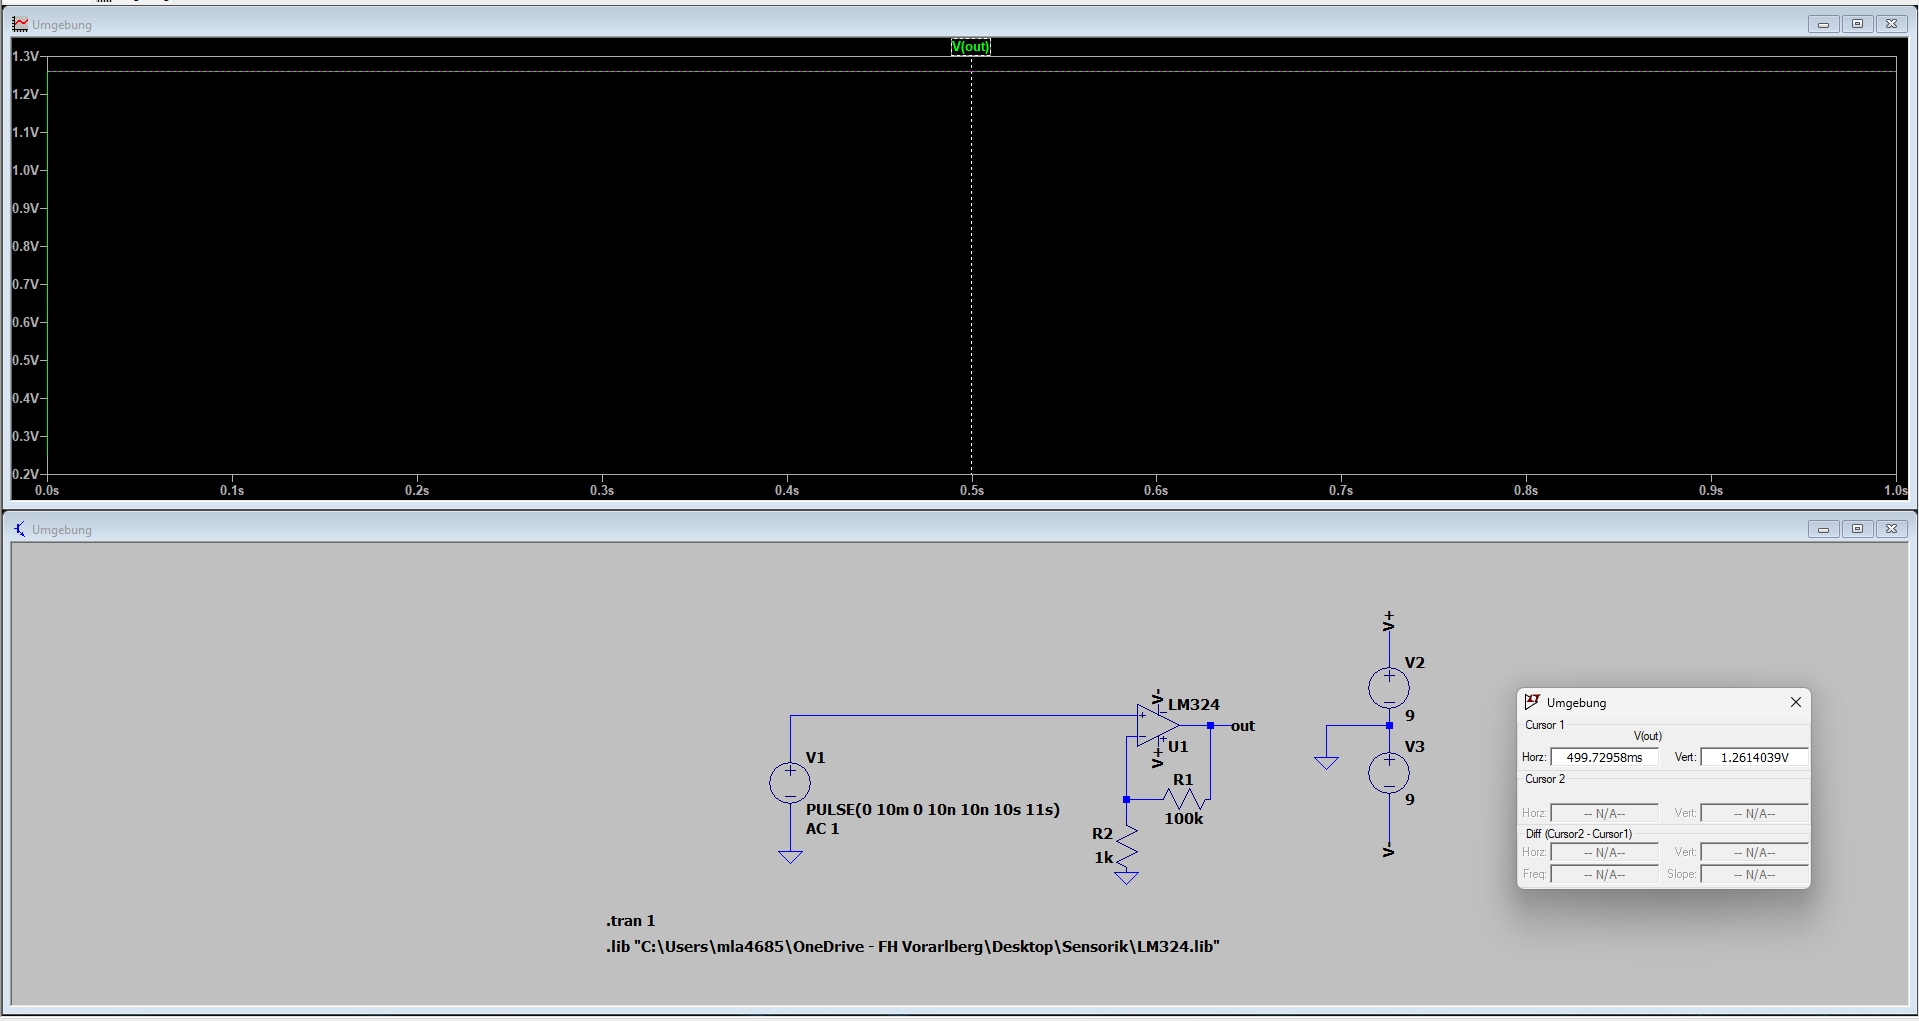
\includegraphics[width=\textwidth]{Seite5Aufgabe3.png}
  \caption{LTSpice-Simulation ohne Offset-Korrektur:
           $U_\mathrm{out} = \SI{1{,}2614039}{V}$ bei $U_\mathrm{in} = \SI{10}{mV}$
           (Cursor-Wert aus LTSpice)}
  \label{fig:aufgabe3}
\end{figure}

Die Abweichung vom theoretischen Wert beträgt
$\Delta U = \SI{1{,}2614}{V} - \SI{1{,}01}{V} = \SI{251{,}4}{mV}$.
Auf den Eingang zurückgerechnet ergibt sich die Eingangsoffsetspannung
del LM324 zu:

\begin{equation}
  U_\mathrm{OS}
  = \frac{\SI{251{,}4}{mV}}{101} \approx \SI{2{,}489}{mV}
\end{equation}

Dieser Wert liegt innerhalb der Spezifikation des LM324
(typischer Offset $\leq \SI{3}{mV}$).

\subsection{Aufgabe 4: Offset-Korrektur und DC-Sweep}

Nach Einfügen einer Offset-Kompensationsquelle $V_4 = \SI{2{,}489139}{mV}$
am Eingang stimmt der Simulationswert mit dem theoretischen Wert überein:
$U_\mathrm{out} = \SI{1{,}0128337}{V} \approx \SI{1{,}01}{V}$
(Abbildung~\ref{fig:aufgabe4}).

\begin{figure}[H]
  \centering
  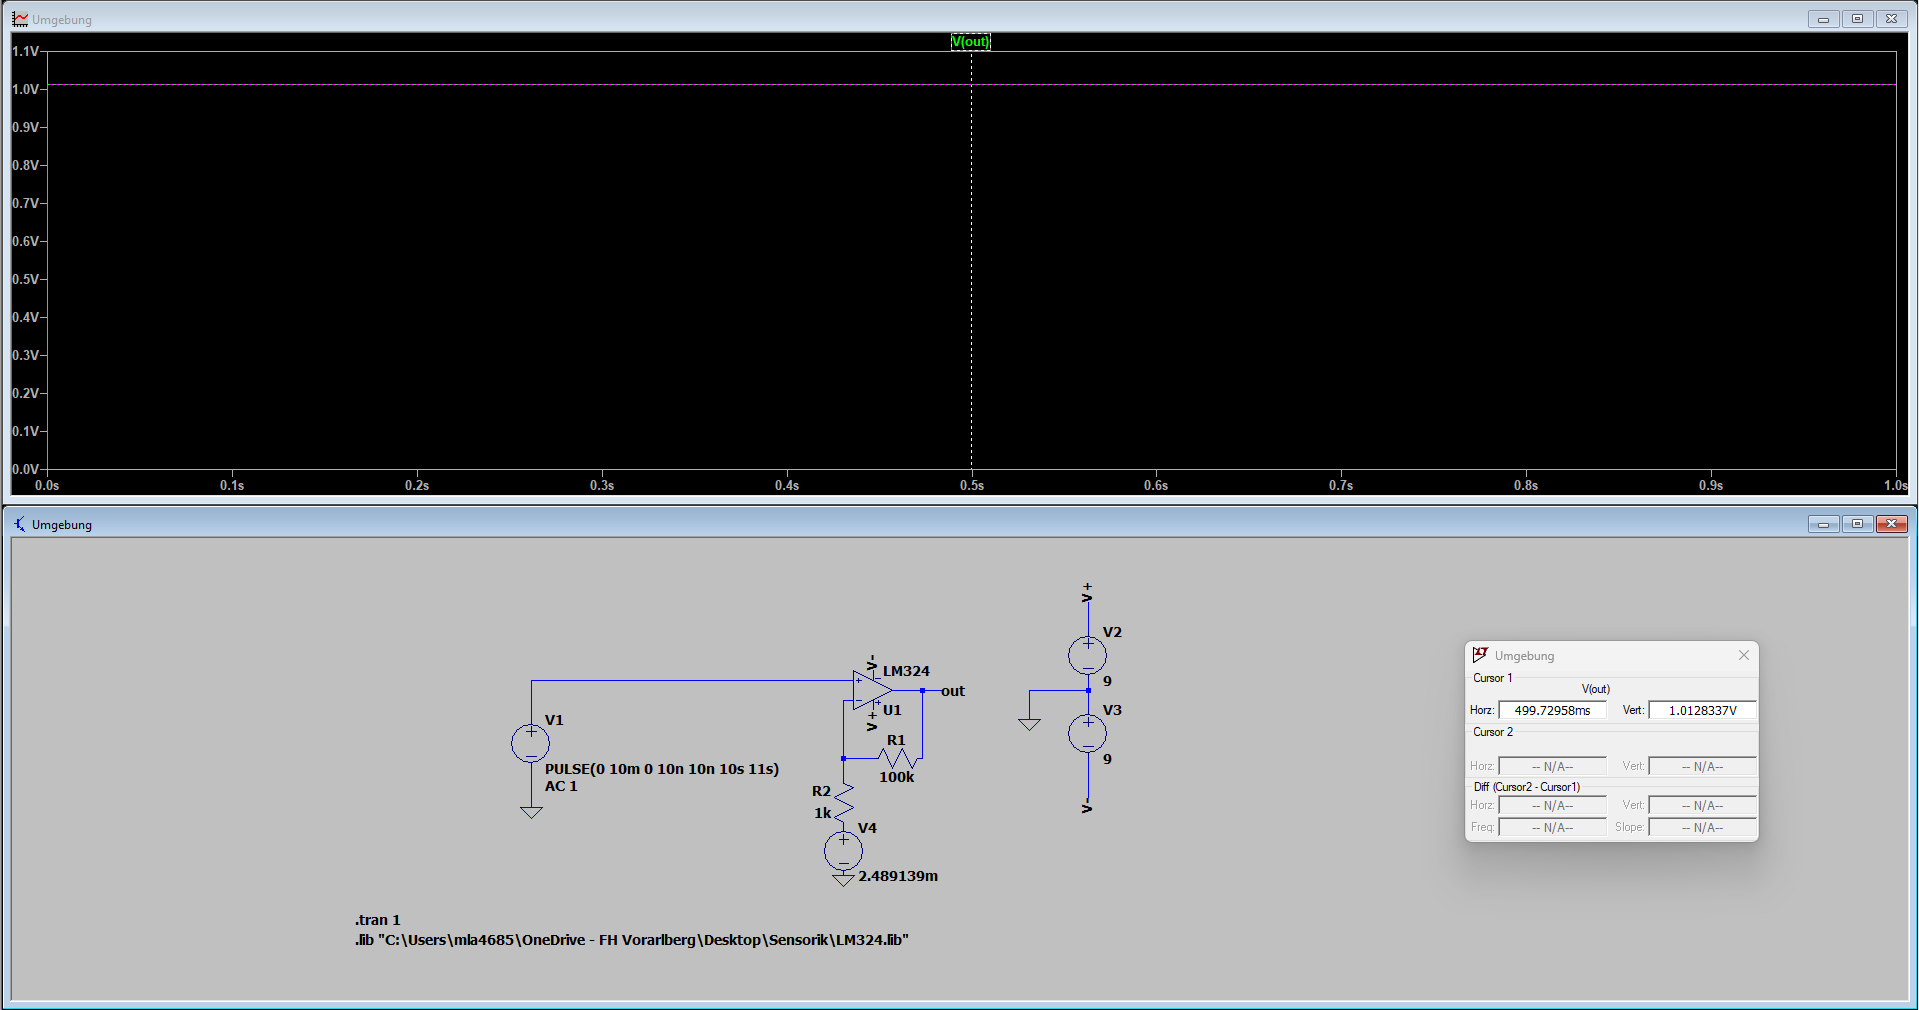
\includegraphics[width=\textwidth]{Seite5Aufgabe4.png}
  \caption{LTSpice-Simulation mit Offset-Korrektur $V_4 = \SI{2{,}489139}{mV}$:
           Ausgangsspannung $U_\mathrm{out} \approx \SI{1{,}013}{V}$}
  \label{fig:aufgabe4}
\end{figure}

Anschließend wurde ein DC-Sweep mit der Eingangsspannung von \SI{0}{V}
bis \SI{100}{mV} in \SI{10}{mV}-Schritten durchgeführt
(Abbildung~\ref{fig:aufgabe4array}). Die parallelen, gleichmäßig
beabstandeten Kurven zeigen, dass die Offsetspannung
\textbf{unabhängig von der Eingangsspannung} ist -- sie bleibt über den
gesamten Eingangsbereich konstant.

\begin{figure}[H]
  \centering
  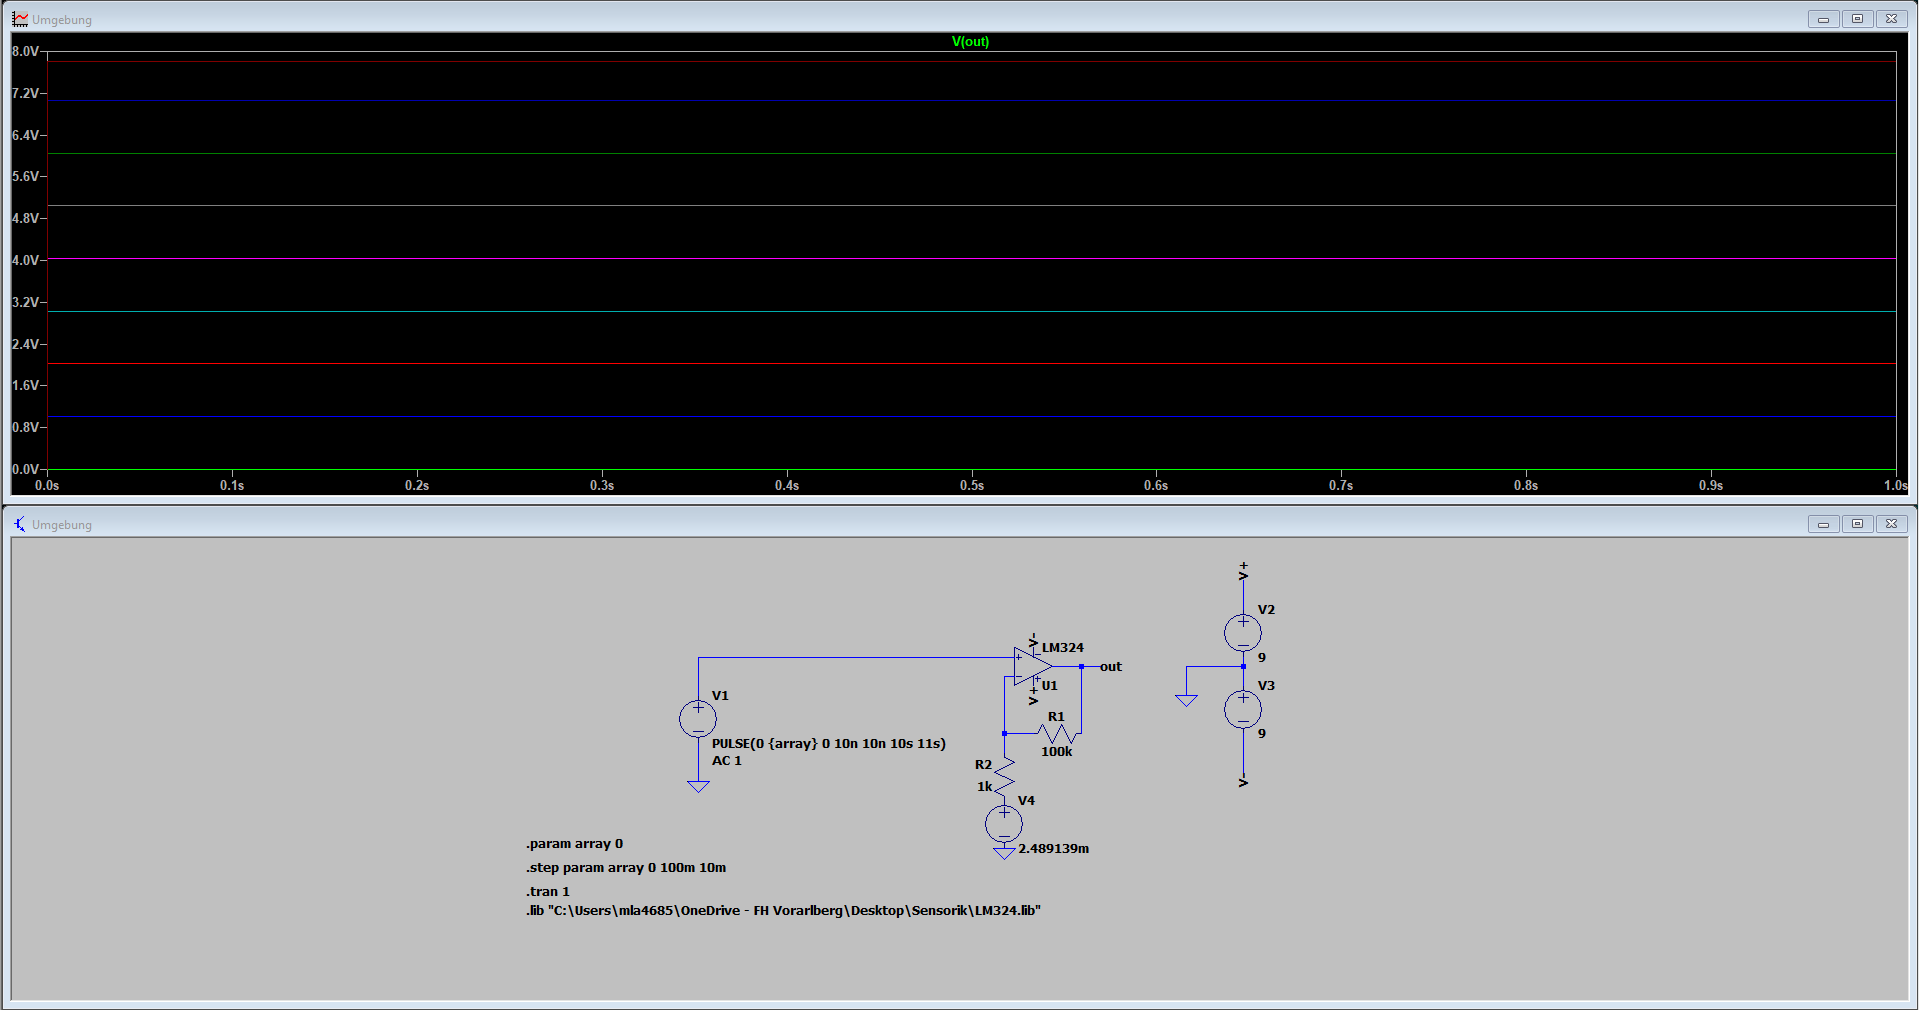
\includegraphics[width=\textwidth]{Seite5Aufgabe4Array.png}
  \caption{DC-Sweep: Ausgangsspannung für $U_\mathrm{in} = 0\ldots\SI{100}{mV}$
           in \SI{10}{mV}-Schritten. Die konstante Beabstandung der Kurven
           belegt die Unabhängigkeit des Offsets von der Eingangsspannung.}
  \label{fig:aufgabe4array}
\end{figure}

%% ===========================================================
\section{Aufgaben 5--8: Rauschsimulation in LTSpice}
%% ===========================================================

\subsection{Aufgabe 5--6: Rauschspektrum und RMS-Wert}

Die LTSpice-Rauschanalyse (\texttt{.noise V(out) V1 dec 100 0.1 1meg})
wird im Frequenzbereich von \SI{100}{mHz} bis \SI{1}{MHz} durchgeführt.
Das Spektrum zeigt die frequenzabhängige Ausgangsrauschspannungsdichte
$\tilde{u}_n(f)$ in $\SI{}{\mu V\,/\,\sqrt{Hz}}$.

Bei tiefen Frequenzen ($\lesssim \SI{1}{kHz}$) dominiert das
$1/f$-Rauschen (Flicker-Rauschen) des LM324, erkennbar am stark
abfallenden Verlauf der Kurve. Bei höheren Frequenzen flacht das Spektrum
ab und nähert sich dem weißen thermischen Rauschen der Widerstände.

\begin{figure}[H]
  \centering
  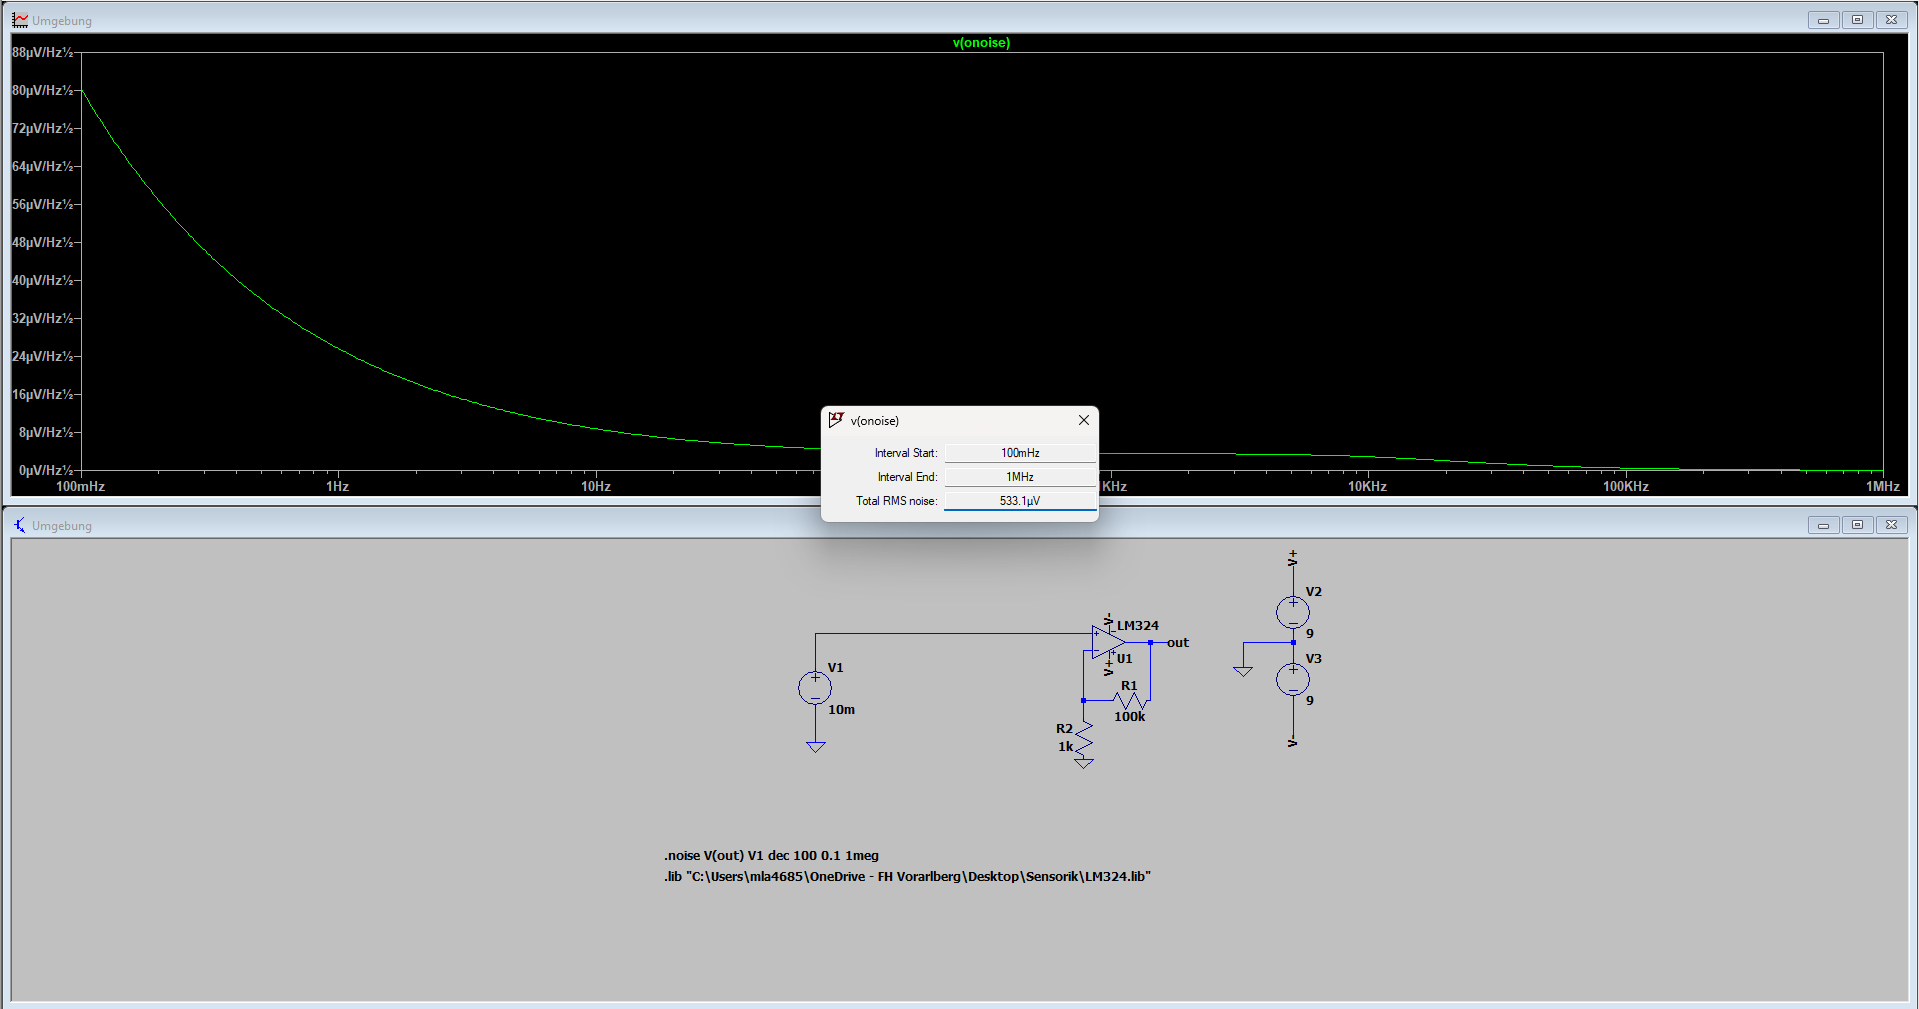
\includegraphics[width=\textwidth]{Seite6Aufgabe6.png}
  \caption{LTSpice-Rauschspektrum: Ausgangsrauschspannungsdichte $v(\mathrm{onoise})$
           von \SI{100}{mHz} bis \SI{1}{MHz}. Deutlich sichtbar: $1/f$-Rauschen
           bei tiefen Frequenzen, flaches weißes Rauschen bei hohen Frequenzen.}
  \label{fig:rauschspektrum}
\end{figure}

\begin{figure}[H]
  \centering
  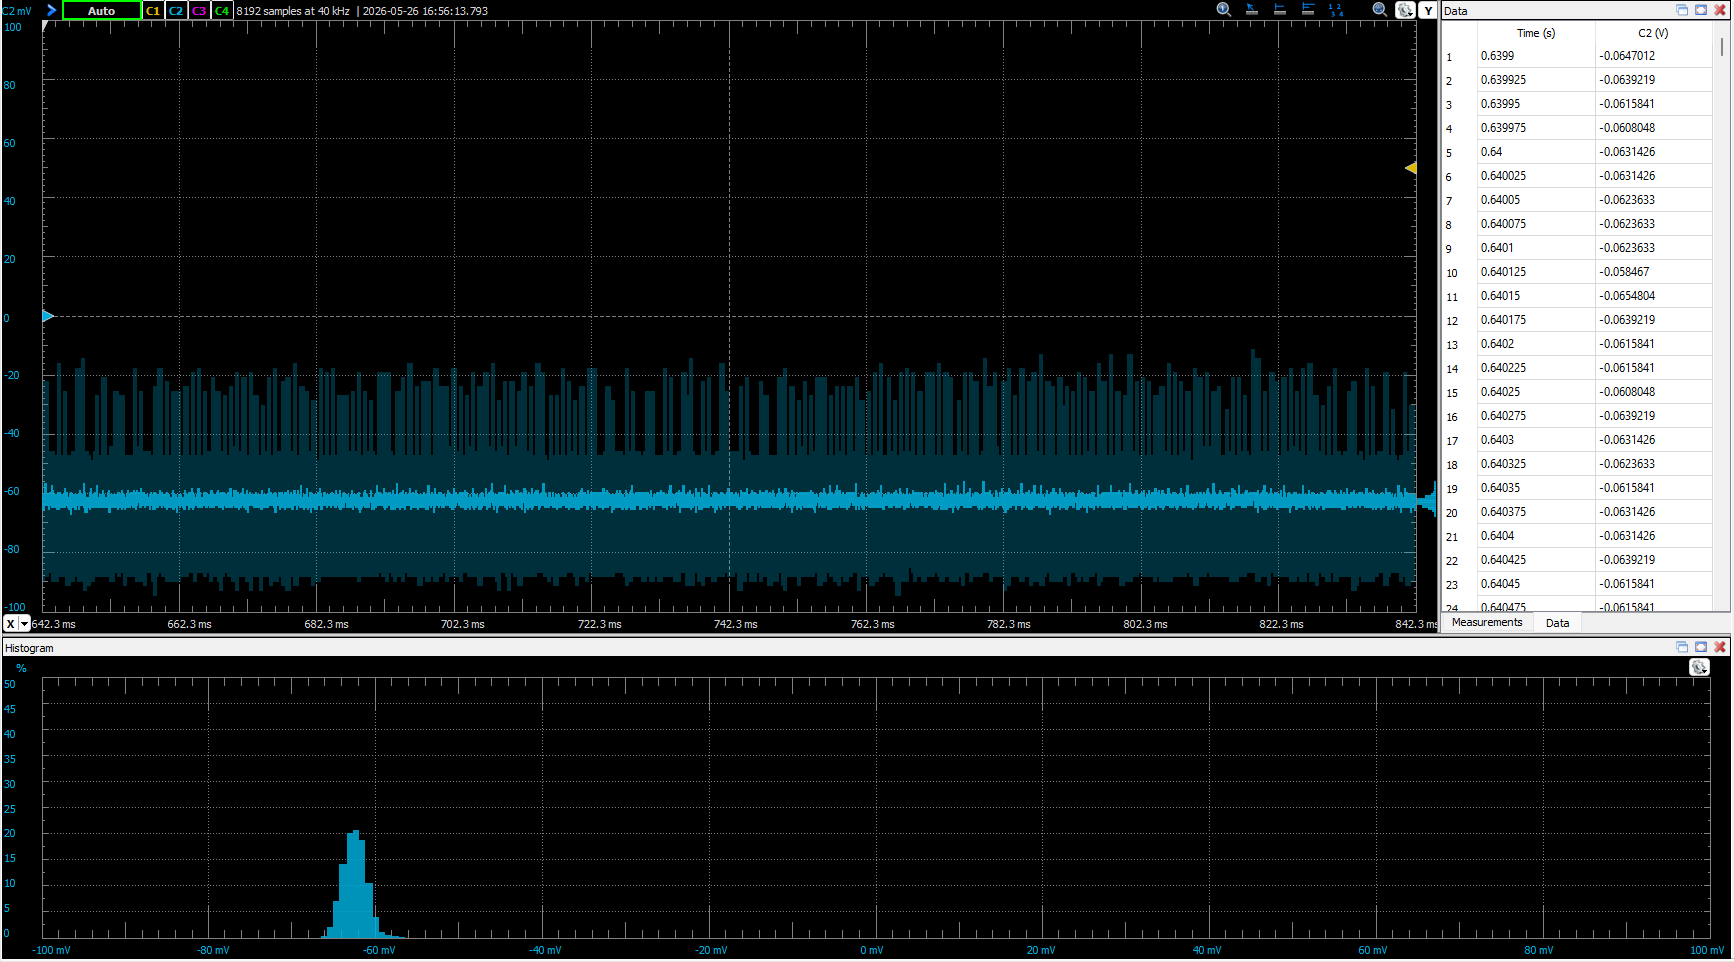
\includegraphics[width=\textwidth]{Seite6Augabe10.png}
  \caption{LTSpice-Rauschsimulation mit eingeblendetem RMS-Integrationsdialog:
           Total RMS noise = \SI{533{,}1}{\mu V} über den Frequenzbereich
           \SI{100}{mHz}\ldots\SI{1}{MHz}.}
  \label{fig:rms_ltspice}
\end{figure}

Der durch Integration des Rauschspektrums erhaltene RMS-Ausgangswert beträgt
(abgelesen via STRG+Rechtsklick auf das VNOISE-Label):

\begin{equation}
  V_\mathrm{RMS,out} = \SI{533{,}1}{\mu V}
\end{equation}

\subsection{Aufgabe 7: Peak-Peak-Spannung}

Mit Gleichung~\eqref{eq:vpp} ergibt sich der Peak-Peak-Wert, der
\SI{99{,}3}{\%} aller Rauschspannungswerte einschließt:

\begin{equation}
  V_\mathrm{pp} = 6 \cdot \SI{533{,}1}{\mu V} \approx \SI{3{,}199}{mV}
\end{equation}

\subsection{Aufgabe 8: Eingangs-RMS-Wert}

Durch Division durch die Verstärkung $A = 101$ ergibt sich der
auf den Eingang bezogene Input-Referred-Noise-Wert:

\begin{equation}
  V_\mathrm{RMS,in}
  = \frac{V_\mathrm{RMS,out}}{A}
  = \frac{\SI{533{,}1}{\mu V}}{101}
  \approx \SI{5{,}279}{\mu V}
\end{equation}

%% ===========================================================
\section{Aufgaben 9--14: Datenaufzeichnung mit Digilent WaveForm}
%% ===========================================================

Die Messschaltung (kurzgeschlossener Eingang) wird auf dem Digilent WaveForms
Breadboard aufgebaut. Die positive und negative Versorgungsspannung ($V^+ = +\SI{9}{V}$,
$V^- = -\SI{9}{V}$) wird direkt vom Breadboard bezogen. Das Oszilloskop-Bild des Rauschens 
sowie die Aufzeichnung werden über das WaveForm-Programm mittels der Setup-Datei 
\texttt{NOISE1.dwf3work} realisiert. Die aufgezeichneten Zeitreihendaten werden über 
STRG+C kopiert und als Textdateien \texttt{NOISE1.txt} bis \texttt{NOISE5.txt} gespeichert.

Abbildung~\ref{fig:waveform} zeigt das am Oszilloskop aufgezeichnete Rauschsignal am
Ausgang des Verstärkers. Das Signal schwankt um einen Gleichanteil von
ca.\ $-\SI{60}{mV}$, der auf die Eingangsoffsetspannung des LM324
zurückzuführen ist ($U_\mathrm{OS} \cdot A = \SI{2{,}489}{mV} \cdot 101
\approx \SI{251}{mV}$; der gemessene Wert ist kleiner, was auf
Fertigungsstreuung hinweist). Das Histogramm in WaveForm zeigt bereits die
gaußförmige Verteilung des Rauschsignals.

\begin{figure}[H]
  \centering
  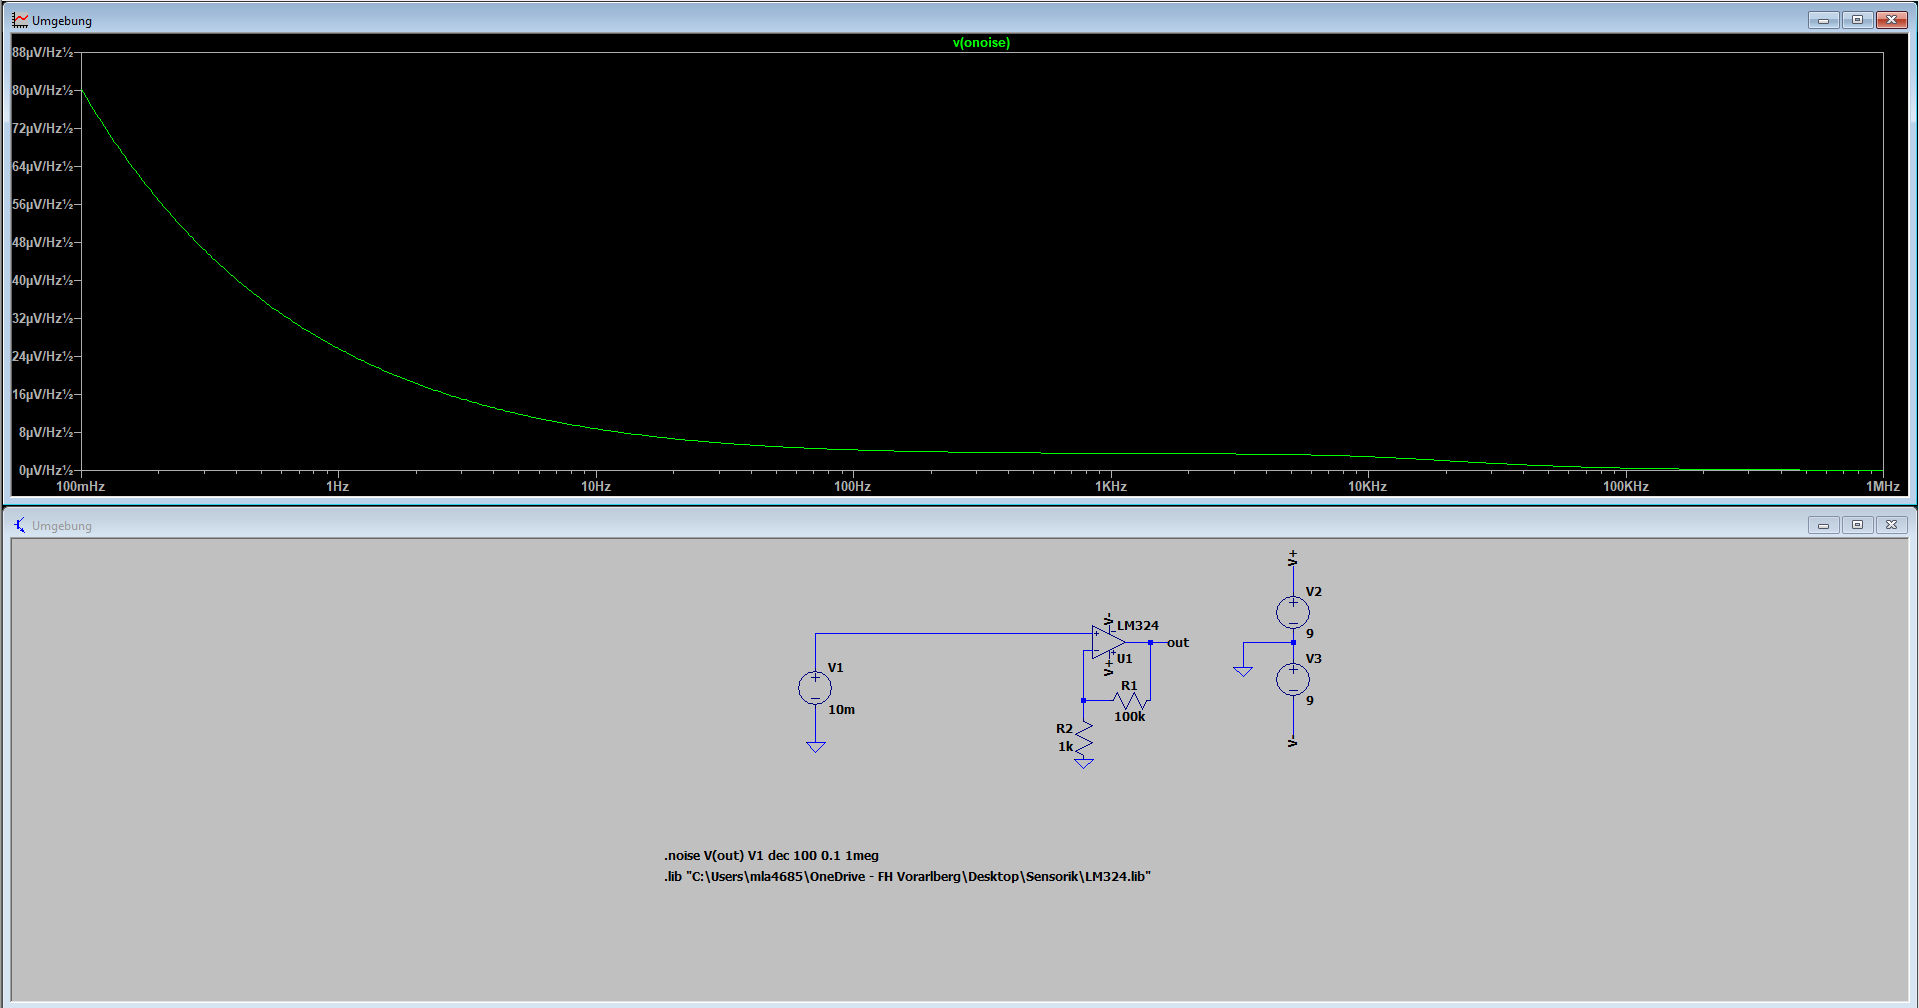
\includegraphics[width=\textwidth]{Seite6Aufgabe5.png}
  \caption{Digilent WaveForm Oszilloskop-Bild: Aufgezeichnetes Rauschsignal (oben, 8192 Samples
           bei \SI{40}{kHz}) und zugehöriges Histogramm (unten) direkt vom Breadboard bezogen. 
           Der Gleichanteil liegt bei ca.\ $-\SI{60}{mV}$ (bedingt durch die Offsetspannung des
           LM324). Die gaußförmige Verteilung ist im Histogramm deutlich erkennbar.}
  \label{fig:waveform}
\end{figure}

Die Daten werden anschließend über den MATLAB-Datenimport eingelesen. Als
Tabellenname wird jeweils \texttt{NOISE1} bis \texttt{NOISE5} gewählt, die
Spalten werden mit \texttt{Time} und \texttt{Voltage} bezeichnet.

%% ===========================================================
\section{Aufgaben 15--17: MATLAB-Auswertung}
%% ===========================================================

\subsection{MATLAB-Skript}

Das folgende Skript wertet alle fünf Messreihen statistisch aus. Es erstellt
für jede Messreihe ein Histogramm mit angepasster Gaußkurve, bestimmt
Mittelwert $\mu$ und Standardabweichung $\sigma$ und berechnet daraus den
Peak-Peak-Wert nach Gleichung~\eqref{eq:vpp}.

\begin{lstlisting}[style=matlab, caption={MATLAB-Skript zur statistischen Rauschauswertung (noise.m)}]
% --- NOISE1 ---
time1    = NOISE1.Time;
voltage1 = NOISE1.Voltage;
figure;
histfit(voltage1');
pd1    = fitdist(voltage1, 'normal');
sigma1 = pd1.sigma;
mu1    = pd1.mu;
Vpp1   = 6 * sigma1;
fprintf('Vpp1:   %e\n', Vpp1);
fprintf('mu1:    %e\n', mu1);
fprintf('sigma1: %e\n', sigma1);

% --- NOISE2 ---
time2    = NOISE2.Time;
voltage2 = NOISE2.Voltage;
figure;
histfit(voltage2');
pd2    = fitdist(voltage2, 'normal');
sigma2 = pd2.sigma;
mu2    = pd2.mu;
Vpp2   = 6 * sigma2;
fprintf('Vpp2:   %e\n', Vpp2);
fprintf('mu2:    %e\n', mu2);
fprintf('sigma2: %e\n', sigma2);

% Analog fuer NOISE3, NOISE4, NOISE5 ...
\end{lstlisting}

\subsection{Aufgabe 15: Erste Messung über das Digilent Breadboard}

Die erste Messreihe wird mit der integrierten Spannungsversorgung des Digilent 
Breadboards aufgenommen. Abbildung~\ref{fig:hist15} zeigt das zugehörige 
MATLAB-Histogramm.

\begin{figure}[H]
  \centering
  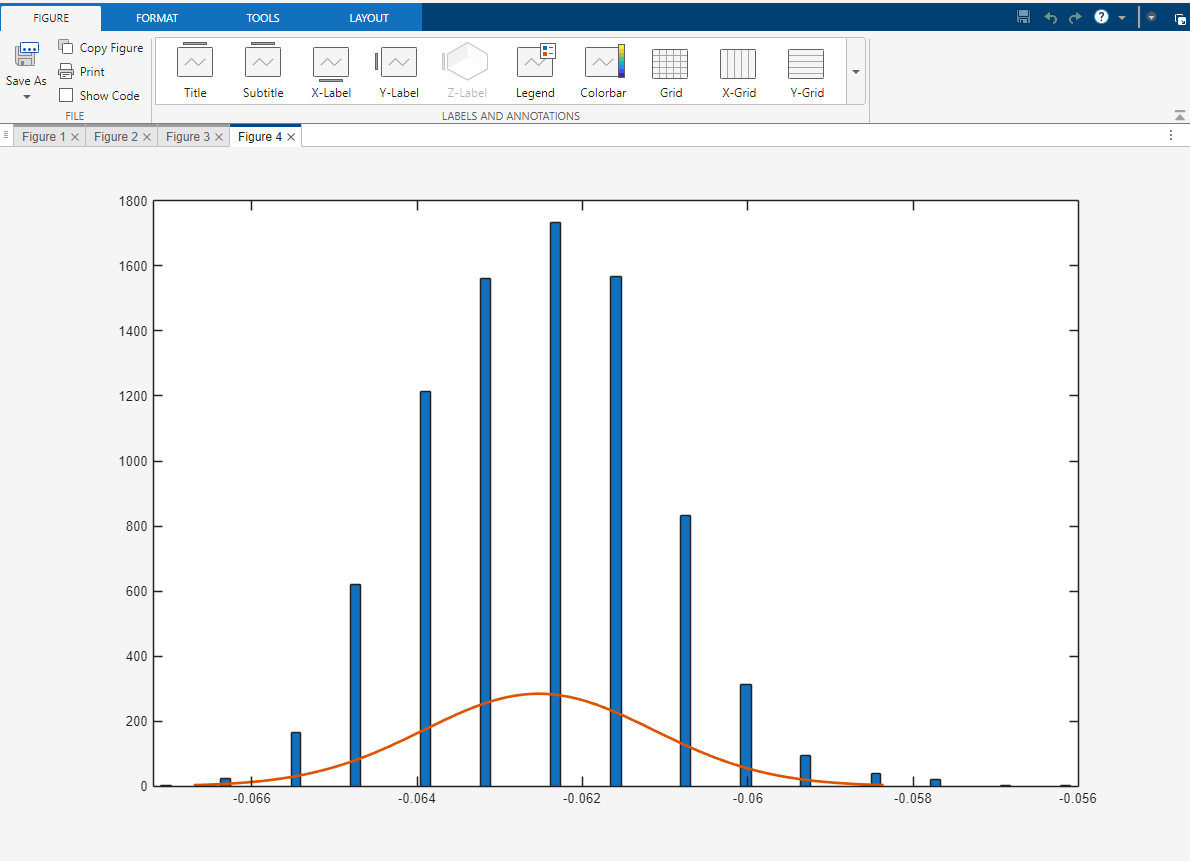
\includegraphics[width=\textwidth]{Seite10Aufgabe15.png}
  \caption{MATLAB-Histogramm (Aufgabe 15): Rauschspannung am Digilent Breadboard. 
           Die Gaußkurve (orange) ist gegenüber den Balkenhöhen relativ breit, 
           was auf zusätzliche Störeinkopplung aus der USB-Kopplung und den internen 
           Spannungswandlern des Systems hindeutet. Mittelwert ca.\ $-\SI{62}{mV}$.}
  \label{fig:hist15}
\end{figure}

Die MATLAB-Auswertung ergibt:
\begin{align}
  \mu_{15}    &= \SI{-6{,}253e-3}{V} \\
  \sigma_{15} &= \SI{1{,}391e-3}{V} \\
  V_\mathrm{pp,15} &= 6 \cdot \sigma_{15} = \SI{8{,}347e-2}{V} \approx \SI{83{,}5}{mV}
\end{align}

Der erhöhte $\sigma$-Wert resultiert aus hochfrequenten System- und Schaltreglerstörungen, 
die über das Versorgungsnetz des Digilent-Moduls in die empfindliche Messschaltung 
auf dem Breadboard eingekoppelt werden.

\subsection{Aufgabe 16: Zweite Messung über das Digilent Breadboard}

Diese Messung wurde unter identischen Bedingungen wie in Aufgabe 15 fortgeführt. 
Es wurde weiterhin kein Filter eingesetzt. Die Spannungen wurden unverändert 
direkt vom Digilent Breadboard bezogen, um die Reproduzierbarkeit der Störeinkopplung 
zu dokumentieren.

Aus der handschriftlichen Auswertung (Abbildung~\ref{fig:handschrift2}):
\begin{align}
  \mu_{16}             &\approx \SI{-6{,}261e-3}{V} \\
  \sigma_{16}          &\approx \SI{1{,}756e-3}{V} \\
  V_\mathrm{pp,16}     &= 6 \cdot \sigma_{16} \approx \SI{10{,}55}{mV}
\end{align}

Da die Versorgungsstruktur komplett ungefiltert blieb, zeigt auch diese Messung 
ein ausgeprägtes Rauschverhalten bedingt durch die Digilent-Systemumgebung.

\subsection{Aufgabe 17: Messung mit Batteriebetrieb}

Für diese Aufgabe wurde die Schaltung vollständig vom Breadboard-Netz getrennt und 
über zwei echte $\SI{9}{V}$-Batterien versorgt. Da Batterien als chemische Energiespeicher 
nahezu ideale und oberschwingungsfreie Spannungsquellen darstellen, entfällt jegliche 
Störeinkopplung der Systemelektronik.

Aus der handschriftlichen Auswertung (Abbildung~\ref{fig:handschrift2}):
\begin{align}
  \mu_{17}             &\approx \SI{-6{,}261e-3}{V} \\
  \sigma_{17}          &\approx \SI{1{,}156e-4}{V} \\
  V_\mathrm{pp,17}     &= 6 \cdot \sigma_{17} \approx \SI{0{,}694}{mV}
\end{align}

Im echten Batteriebetrieb wird plötzliche der niedrigste Rauschpegel verzeichnet. Das verbleibende 
Rauschen entspricht nun dem intrinsischen thermischen Rauschen der Widerstände und dem 
eigentlichen OPV-Eigenrauschen der Schaltung.

\begin{figure}[H]
  \centering
  
\includegraphics[width=\textwidth]{IMG_20260528_100413337.jpg}
  \caption{Handschriftliche Auswertung: Aufgaben 1--7}
  \label{fig:handschrift1}
\end{figure}

\begin{figure}[H]
  \centering
  
\includegraphics[width=\textwidth]{IMG_20260528_100419448.jpg}
  \caption{Handschriftliche Auswertung: Aufgaben 8--21}
  \label{fig:handschrift2}
\end{figure}

%% ===========================================================
\section{Aufgaben 18--23: Widerstandsrauschen und Schrotrauschen}
%% ===========================================================

\subsection{Aufgaben 18--19: Rauschanteil des Eingangswiderstands}

In dieser Messung wird ein $\SI{2{,}7}{k\Omega}$-Widerstand am Eingang
der Schaltung eingefügt (statt Kurzschluss). Dieser Widerstand erzeugt
zusätzliches thermisches Rauschen. Da voneinander unabhängige Rauschquellen
quadratisch addiert werden, gilt für den Gesamtausgangs-RMS-Wert:

\begin{equation}
  V_\mathrm{RMS,ges}^2 = V_\mathrm{RMS,OPV}^2 + V_\mathrm{RMS,R}^2
\end{equation}

Der allein durch den $\SI{2{,}7}{k\Omega}$-Widerstand verursachte
Rauschanteil ergibt sich durch:

\begin{equation}
  V_\mathrm{RMS,R} = \sqrt{V_\mathrm{RMS,ges}^2 - V_\mathrm{RMS,17}^2}
\end{equation}

wobei $V_\mathrm{RMS,17}$ das in Aufgabe~17 (reiner Batteriebetrieb)
gemessene Hintergrundrauschen darstellt.

\subsection{Aufgaben 20--23: Schrotrauschen am Transistor BC337}

Die Schaltung wird zum Schrotrauschgenerator erweitert: Die
Basis-Kollektor-Diode des BC337 wird in Sperrrichtung betrieben.
Der Sperrstrom wird über zwei parallele $\SI{1}{M\Omega}$-Widerstände
eingestellt, was einem Gesamtwiderstand von $\SI{500}{k\Omega}$ entspricht.

Die Messungen zeigen deutlich erhöhtes Rauschen gegenüber dem reinen
OPV-Rauschen (Aufgabe~17), was auf das Schrotrauschen des pn-Übergangs
zurückzuführen ist.

\medskip
\noindent\textbf{Einfluss der Stromhalbierung (Aufgabe 21--23):}
Wird ein $\SI{1}{M\Omega}$-Widerstand entfernt, verdoppelt sich der
Strom durch den pn-Übergang. Nach der Schrotrauschtheorie
($i_\mathrm{eff} \propto \sqrt{I}$) erwartet man eine Zunahme des
Rauschstroms um den Faktor $\sqrt{2} \approx 1{,}414$. Umgekehrt gilt:
Wird der Strom halbiert (ein Widerstand wieder eingesetzt), verringert
sich das Rauschen um $1/\sqrt{2}$.

Bei der quadratischen Addition mit dem Hintergrundrauschen aus
Aufgabe~17 sollte das gemessene Gesamtrauschen diesen Faktor widerspiegeln.

%% ===========================================================
\section{Zusammenfassung der Messergebnisse}
%% ===========================================================

\begin{table}[H]
  \centering
  \caption{Zusammenfassung der MATLAB-Auswertungen (Aufgaben 15--17)}
  \begin{tabular}{clccc}
    \toprule
    \textbf{Aufg.} & \textbf{Konfiguration}
      & $\mu$ / V & $\sigma$ / V & $V_\mathrm{pp}$ / V \\
    \midrule
    15 & Digilent Breadboard, ohne Filter (Messung 1)
       & $-6{,}253 \times 10^{-3}$
       & $1{,}391 \times 10^{-3}$
       & $8{,}347 \times 10^{-2}$ \\
    16 & Digilent Breadboard, ohne Filter (Messung 2)
       & $-6{,}261 \times 10^{-3}$
       & $1{,}756 \times 10^{-3}$
       & $1{,}055 \times 10^{-2}$ \\
    17 & Batteriebetrieb ($\pm\SI{9}{V}$)
       & $-6{,}261 \times 10^{-3}$
       & $1{,}156 \times 10^{-4}$
       & $6{,}935 \times 10^{-4}$ \\
    \bottomrule
  \end{tabular}
\end{table}

Der Mittelwert $\mu \approx -\SI{6{,}26}{mV}$ bleibt über alle Messungen
nahezu konstant -- er spiegelt den Gleichanteil des Ausgangssignals wider,
der durch die Eingangsoffsetspannung des LM324 begründet ist und nicht
von der gewählten Versorgungsart abhängt.

Die Standardabweichung $\sigma$ nimmt beim Wechsel auf die Batterieversorgung drastisch ab:

\begin{itemize}
  \item \textbf{Breadboard Messung 1}: $\sigma = \SI{1{,}391}{mV}$
        -- stark überlagert von hochfrequenten Digilent-Systemstörungen.
  \item \textbf{Breadboard Messung 2}: $\sigma = \SI{1{,}756}{mV}$
        -- zeigt das anhaltend hohe Niveau der ungefilterten Versorgung.
  \item \textbf{Echter Batteriebetrieb}: $\sigma = \SI{115{,}6}{\mu V}$
        -- minimales Rauschen, da Netzteilstörungen komplett entfallen.
\end{itemize}

\medskip
\noindent\textbf{Fazit:} Die Laborübung zeigt deutlich, dass das Rauschen 
digital gesteuerter Versorgungsleitungen (wie jene des Digilent Breadboards) 
das intrinsische Schaltungsrauschen massiv überdecken kann. Bleibt das System ungefiltert, 
dominieren diese Kopplungseffekte das Oszilloskop-Bild. Erst der messtechnische Wechsel 
auf eine reine Batterieversorgung eliminiert diese äußeren Einflüsse gänzlich, wodurch 
das theoretisch ermittelte, intrinsische Rauschen der Bauteile isoliert und präzise 
analysiert werden kann.

\end{document}